\documentclass[twoside]{book}

% Packages required by doxygen
\usepackage{fixltx2e}
\usepackage{calc}
\usepackage{doxygen}
\usepackage{graphicx}
\usepackage[utf8]{inputenc}
\usepackage{makeidx}
\usepackage{multicol}
\usepackage{multirow}
\PassOptionsToPackage{warn}{textcomp}
\usepackage{textcomp}
\usepackage[nointegrals]{wasysym}
\usepackage[table]{xcolor}

% Font selection
\usepackage[T1]{fontenc}
\usepackage{mathptmx}
\usepackage[scaled=.90]{helvet}
\usepackage{courier}
\usepackage{amssymb}
\usepackage{sectsty}
\renewcommand{\familydefault}{\sfdefault}
\allsectionsfont{%
  \fontseries{bc}\selectfont%
  \color{darkgray}%
}
\renewcommand{\DoxyLabelFont}{%
  \fontseries{bc}\selectfont%
  \color{darkgray}%
}
\newcommand{\+}{\discretionary{\mbox{\scriptsize$\hookleftarrow$}}{}{}}

% Page & text layout
\usepackage{geometry}
\geometry{%
  a4paper,%
  top=2.5cm,%
  bottom=2.5cm,%
  left=2.5cm,%
  right=2.5cm%
}
\tolerance=750
\hfuzz=15pt
\hbadness=750
\setlength{\emergencystretch}{15pt}
\setlength{\parindent}{0cm}
\setlength{\parskip}{0.2cm}
\makeatletter
\renewcommand{\paragraph}{%
  \@startsection{paragraph}{4}{0ex}{-1.0ex}{1.0ex}{%
    \normalfont\normalsize\bfseries\SS@parafont%
  }%
}
\renewcommand{\subparagraph}{%
  \@startsection{subparagraph}{5}{0ex}{-1.0ex}{1.0ex}{%
    \normalfont\normalsize\bfseries\SS@subparafont%
  }%
}
\makeatother

% Headers & footers
\usepackage{fancyhdr}
\pagestyle{fancyplain}
\fancyhead[LE]{\fancyplain{}{\bfseries\thepage}}
\fancyhead[CE]{\fancyplain{}{}}
\fancyhead[RE]{\fancyplain{}{\bfseries\leftmark}}
\fancyhead[LO]{\fancyplain{}{\bfseries\rightmark}}
\fancyhead[CO]{\fancyplain{}{}}
\fancyhead[RO]{\fancyplain{}{\bfseries\thepage}}
\fancyfoot[LE]{\fancyplain{}{}}
\fancyfoot[CE]{\fancyplain{}{}}
\fancyfoot[RE]{\fancyplain{}{\bfseries\scriptsize Generated on Sun Apr 3 2016 12\+:44\+:44 for My Project by Doxygen }}
\fancyfoot[LO]{\fancyplain{}{\bfseries\scriptsize Generated on Sun Apr 3 2016 12\+:44\+:44 for My Project by Doxygen }}
\fancyfoot[CO]{\fancyplain{}{}}
\fancyfoot[RO]{\fancyplain{}{}}
\renewcommand{\footrulewidth}{0.4pt}
\renewcommand{\chaptermark}[1]{%
  \markboth{#1}{}%
}
\renewcommand{\sectionmark}[1]{%
  \markright{\thesection\ #1}%
}

% Indices & bibliography
\usepackage{natbib}
\usepackage[titles]{tocloft}
\setcounter{tocdepth}{3}
\setcounter{secnumdepth}{5}
\makeindex

% Hyperlinks (required, but should be loaded last)
\usepackage{ifpdf}
\ifpdf
  \usepackage[pdftex,pagebackref=true]{hyperref}
\else
  \usepackage[ps2pdf,pagebackref=true]{hyperref}
\fi
\hypersetup{%
  colorlinks=true,%
  linkcolor=blue,%
  citecolor=blue,%
  unicode%
}

% Custom commands
\newcommand{\clearemptydoublepage}{%
  \newpage{\pagestyle{empty}\cleardoublepage}%
}


%===== C O N T E N T S =====

\begin{document}

% Titlepage & ToC
\hypersetup{pageanchor=false,
             bookmarks=true,
             bookmarksnumbered=true,
             pdfencoding=unicode
            }
\pagenumbering{roman}
\begin{titlepage}
\vspace*{7cm}
\begin{center}%
{\Large My Project }\\
\vspace*{1cm}
{\large Generated by Doxygen 1.8.7}\\
\vspace*{0.5cm}
{\small Sun Apr 3 2016 12:44:44}\\
\end{center}
\end{titlepage}
\clearemptydoublepage
\tableofcontents
\clearemptydoublepage
\pagenumbering{arabic}
\hypersetup{pageanchor=true}

%--- Begin generated contents ---
\chapter{Class Index}
\section{Class List}
Here are the classes, structs, unions and interfaces with brief descriptions\+:\begin{DoxyCompactList}
\item\contentsline{section}{\hyperlink{struct__Mensaje}{\+\_\+\+Mensaje} \\*Mensaje }{\pageref{struct__Mensaje}}{}
\item\contentsline{section}{\hyperlink{structAula}{Aula} \\*\hyperlink{structAula}{Aula} }{\pageref{structAula}}{}
\end{DoxyCompactList}

\chapter{File Index}
\section{File List}
Here is a list of all documented files with brief descriptions\+:\begin{DoxyCompactList}
\item\contentsline{section}{\hyperlink{ej4a_8c}{ej4a.\+c} \\*El ejercicio 4a de la Practica 1 S\+O\+P\+E\+R }{\pageref{ej4a_8c}}{}
\item\contentsline{section}{\hyperlink{ej4b_8c}{ej4b.\+c} \\*El ejercicio 4b de la Practica 1 S\+O\+P\+E\+R }{\pageref{ej4b_8c}}{}
\item\contentsline{section}{\hyperlink{ej5a_8c}{ej5a.\+c} \\*El ejercicio 5a de la Practica 1 S\+O\+P\+E\+R }{\pageref{ej5a_8c}}{}
\item\contentsline{section}{\hyperlink{ej5b_8c}{ej5b.\+c} \\*El ejercicio 5b de la Practica 1 S\+O\+P\+E\+R }{\pageref{ej5b_8c}}{}
\item\contentsline{section}{\hyperlink{ej8a_8c}{ej8a.\+c} \\*El ejercicio 8a de la Practica 1 S\+O\+P\+E\+R }{\pageref{ej8a_8c}}{}
\item\contentsline{section}{\hyperlink{ej8b_8c}{ej8b.\+c} \\*El ejercicio 8b de la Practica 1 S\+O\+P\+E\+R }{\pageref{ej8b_8c}}{}
\item\contentsline{section}{\hyperlink{ejercicio6_8c}{ejercicio6.\+c} \\*El ejercicio 6 de la Practica 1 S\+O\+P\+E\+R }{\pageref{ejercicio6_8c}}{}
\item\contentsline{section}{\hyperlink{ejercicio9_8c}{ejercicio9.\+c} \\*El ejercicio 9 de la Practica 1 S\+O\+P\+E\+R }{\pageref{ejercicio9_8c}}{}
\end{DoxyCompactList}

\chapter{Class Documentation}
\hypertarget{structinfo}{\section{info Struct Reference}
\label{structinfo}\index{info@{info}}
}


Variables compartidas.  


\subsection*{Public Attributes}
\begin{DoxyCompactItemize}
\item 
\hypertarget{structinfo_aaa02777b492865c2877852cb159803b1}{char {\bfseries nombre} \mbox{[}80\mbox{]}}\label{structinfo_aaa02777b492865c2877852cb159803b1}

\item 
\hypertarget{structinfo_afe86f23d8bd5fd8d139e39a5b1a01171}{int {\bfseries id}}\label{structinfo_afe86f23d8bd5fd8d139e39a5b1a01171}

\item 
int \hyperlink{structinfo_abf4c654e057e50646e8a3cd5ecf67a76}{c\+Va}
\item 
int \hyperlink{structinfo_a95e1221a8023ea0ec9b94d0795a6f139}{c\+Vi}
\end{DoxyCompactItemize}


\subsection{Detailed Description}
Variables compartidas. 

Esta estructura sirve para poder compartir variables entre procesos 

\subsection{Member Data Documentation}
\hypertarget{structinfo_abf4c654e057e50646e8a3cd5ecf67a76}{\index{info@{info}!c\+Va@{c\+Va}}
\index{c\+Va@{c\+Va}!info@{info}}
\subsubsection[{c\+Va}]{\setlength{\rightskip}{0pt plus 5cm}int info\+::c\+Va}}\label{structinfo_abf4c654e057e50646e8a3cd5ecf67a76}
cuenta Va \hypertarget{structinfo_a95e1221a8023ea0ec9b94d0795a6f139}{\index{info@{info}!c\+Vi@{c\+Vi}}
\index{c\+Vi@{c\+Vi}!info@{info}}
\subsubsection[{c\+Vi}]{\setlength{\rightskip}{0pt plus 5cm}int info\+::c\+Vi}}\label{structinfo_a95e1221a8023ea0ec9b94d0795a6f139}
cuenta Vi 

The documentation for this struct was generated from the following files\+:\begin{DoxyCompactItemize}
\item 
\hyperlink{ejercicio2_8c}{ejercicio2.\+c}\item 
\hyperlink{ejercicio6_8c}{ejercicio6.\+c}\end{DoxyCompactItemize}

\chapter{File Documentation}
\hypertarget{ejercicio2_8c}{\section{ejercicio2.\+c File Reference}
\label{ejercicio2_8c}\index{ejercicio2.\+c@{ejercicio2.\+c}}
}


El ejercicio 2 de la Practica 3 S\+O\+P\+E\+R.  


{\ttfamily \#include $<$stdio.\+h$>$}\\*
{\ttfamily \#include $<$stdlib.\+h$>$}\\*
{\ttfamily \#include $<$string.\+h$>$}\\*
{\ttfamily \#include $<$sys/wait.\+h$>$}\\*
{\ttfamily \#include $<$sys/types.\+h$>$}\\*
{\ttfamily \#include $<$sys/ipc.\+h$>$}\\*
{\ttfamily \#include $<$errno.\+h$>$}\\*
{\ttfamily \#include $<$sys/shm.\+h$>$}\\*
{\ttfamily \#include $<$signal.\+h$>$}\\*
Include dependency graph for ejercicio2.\+c\+:
\nopagebreak
\begin{figure}[H]
\begin{center}
\leavevmode
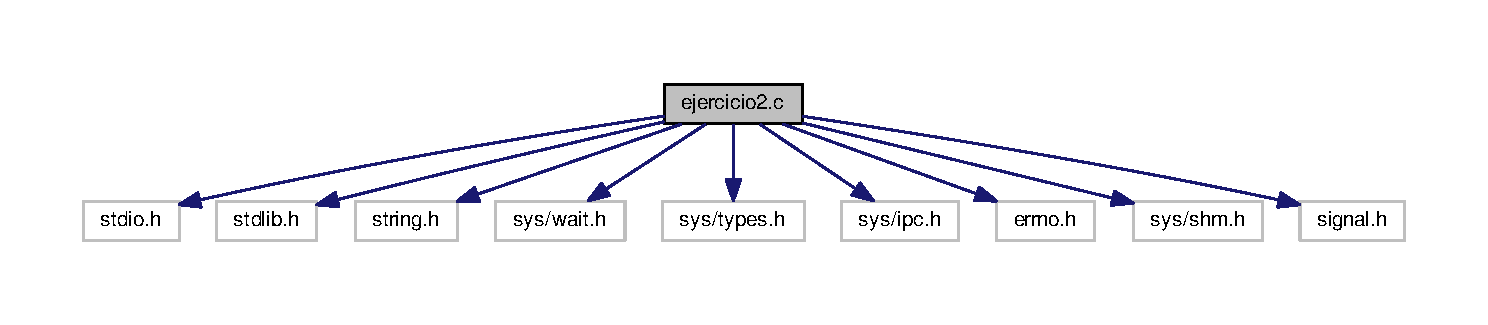
\includegraphics[width=350pt]{ejercicio2_8c__incl}
\end{center}
\end{figure}
\subsection*{Classes}
\begin{DoxyCompactItemize}
\item 
struct \hyperlink{structinfo}{info}
\begin{DoxyCompactList}\small\item\em Variables compartidas. \end{DoxyCompactList}\end{DoxyCompactItemize}
\subsection*{Macros}
\begin{DoxyCompactItemize}
\item 
\hypertarget{ejercicio2_8c_a68c15c5fb7f7c6f707903e6a46ab0557}{\#define {\bfseries F\+I\+L\+E\+K\+E\+Y}~\char`\"{}/bin/cat\char`\"{}}\label{ejercicio2_8c_a68c15c5fb7f7c6f707903e6a46ab0557}

\item 
\hypertarget{ejercicio2_8c_a8ae9d53f33f46cfcfcb9736e6351452a}{\#define {\bfseries K\+E\+Y}~1300}\label{ejercicio2_8c_a8ae9d53f33f46cfcfcb9736e6351452a}

\end{DoxyCompactItemize}
\subsection*{Functions}
\begin{DoxyCompactItemize}
\item 
void \hyperlink{ejercicio2_8c_af67f7ad6bdff3c40a6b1d97ae573fa4c}{manejador\+\_\+\+S\+I\+G\+U\+S\+R1} (int sig)
\begin{DoxyCompactList}\small\item\em manejador\+\_\+\+S\+I\+G\+U\+S\+R1 Imprime por pantalla el contenido del buffer \end{DoxyCompactList}\item 
int \hyperlink{ejercicio2_8c_a0ddf1224851353fc92bfbff6f499fa97}{main} (int argc, char $\ast$argv\mbox{[}$\,$\mbox{]})
\begin{DoxyCompactList}\small\item\em Varios procesos usan memoria compartida Un proceso padre lee el contenido de la memoria compartida tras recibir una señal de sus procesos hijos que escriben en esa memoria. \end{DoxyCompactList}\end{DoxyCompactItemize}
\subsection*{Variables}
\begin{DoxyCompactItemize}
\item 
\hypertarget{ejercicio2_8c_a52b5a4f82d3598ac1e6ab6d145ce72a4}{struct \hyperlink{structinfo}{info} $\ast$ {\bfseries buffer}}\label{ejercicio2_8c_a52b5a4f82d3598ac1e6ab6d145ce72a4}

\end{DoxyCompactItemize}


\subsection{Detailed Description}
El ejercicio 2 de la Practica 3 S\+O\+P\+E\+R. 

\begin{DoxyAuthor}{Author}
Oscar Garcia de Lara Parreño 

Santiago Gomez Aguirre 
\end{DoxyAuthor}
\begin{DoxyVersion}{Version}
1.\+0 
\end{DoxyVersion}
\begin{DoxyDate}{Date}
10-\/03-\/2016 
\end{DoxyDate}


\subsection{Function Documentation}
\hypertarget{ejercicio2_8c_a0ddf1224851353fc92bfbff6f499fa97}{\index{ejercicio2.\+c@{ejercicio2.\+c}!main@{main}}
\index{main@{main}!ejercicio2.\+c@{ejercicio2.\+c}}
\subsubsection[{main}]{\setlength{\rightskip}{0pt plus 5cm}int main (
\begin{DoxyParamCaption}
\item[{int}]{argc, }
\item[{char $\ast$}]{argv\mbox{[}$\,$\mbox{]}}
\end{DoxyParamCaption}
)}}\label{ejercicio2_8c_a0ddf1224851353fc92bfbff6f499fa97}


Varios procesos usan memoria compartida Un proceso padre lee el contenido de la memoria compartida tras recibir una señal de sus procesos hijos que escriben en esa memoria. 

\begin{DoxyReturn}{Returns}
E\+X\+I\+T\+\_\+\+F\+A\+I\+L\+U\+R\+E en caso de error, E\+X\+I\+T\+\_\+\+S\+U\+C\+C\+E\+S\+S si funciona 
\end{DoxyReturn}
\hypertarget{ejercicio2_8c_af67f7ad6bdff3c40a6b1d97ae573fa4c}{\index{ejercicio2.\+c@{ejercicio2.\+c}!manejador\+\_\+\+S\+I\+G\+U\+S\+R1@{manejador\+\_\+\+S\+I\+G\+U\+S\+R1}}
\index{manejador\+\_\+\+S\+I\+G\+U\+S\+R1@{manejador\+\_\+\+S\+I\+G\+U\+S\+R1}!ejercicio2.\+c@{ejercicio2.\+c}}
\subsubsection[{manejador\+\_\+\+S\+I\+G\+U\+S\+R1}]{\setlength{\rightskip}{0pt plus 5cm}void manejador\+\_\+\+S\+I\+G\+U\+S\+R1 (
\begin{DoxyParamCaption}
\item[{int}]{sig}
\end{DoxyParamCaption}
)}}\label{ejercicio2_8c_af67f7ad6bdff3c40a6b1d97ae573fa4c}


manejador\+\_\+\+S\+I\+G\+U\+S\+R1 Imprime por pantalla el contenido del buffer 


\begin{DoxyParams}{Parameters}
{\em sig} & Señal de entrada \\
\hline
\end{DoxyParams}

\hypertarget{ejercicio5_8c}{\section{ejercicio5.\+c File Reference}
\label{ejercicio5_8c}\index{ejercicio5.\+c@{ejercicio5.\+c}}
}


El ejercicio 5 de la Practica 3 S\+O\+P\+E\+R.  


{\ttfamily \#include $<$string.\+h$>$}\\*
{\ttfamily \#include $<$signal.\+h$>$}\\*
{\ttfamily \#include \char`\"{}semaforos.\+h\char`\"{}}\\*
Include dependency graph for ejercicio5.\+c\+:
\nopagebreak
\begin{figure}[H]
\begin{center}
\leavevmode
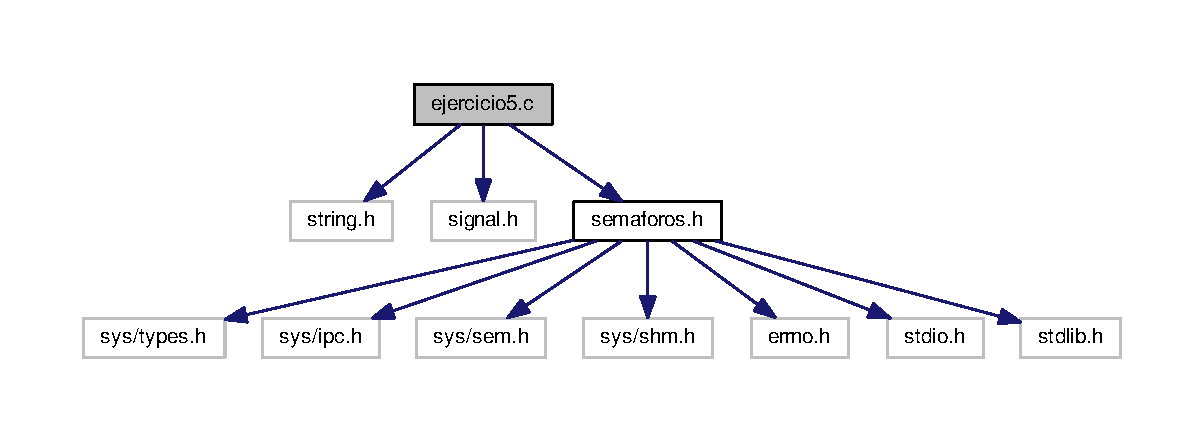
\includegraphics[width=350pt]{ejercicio5_8c__incl}
\end{center}
\end{figure}
\subsection*{Macros}
\begin{DoxyCompactItemize}
\item 
\hypertarget{ejercicio5_8c_a0240ac851181b84ac374872dc5434ee4}{\#define {\bfseries N}~100}\label{ejercicio5_8c_a0240ac851181b84ac374872dc5434ee4}

\item 
\hypertarget{ejercicio5_8c_a68c15c5fb7f7c6f707903e6a46ab0557}{\#define {\bfseries F\+I\+L\+E\+K\+E\+Y}~\char`\"{}/bin/cat\char`\"{}}\label{ejercicio5_8c_a68c15c5fb7f7c6f707903e6a46ab0557}

\end{DoxyCompactItemize}
\subsection*{Typedefs}
\begin{DoxyCompactItemize}
\item 
\hypertarget{ejercicio5_8c_a081a8c30a2974cba7f7e1a1569c8d0ba}{typedef int {\bfseries item}}\label{ejercicio5_8c_a081a8c30a2974cba7f7e1a1569c8d0ba}

\end{DoxyCompactItemize}
\subsection*{Functions}
\begin{DoxyCompactItemize}
\item 
int \hyperlink{ejercicio5_8c_a0ddf1224851353fc92bfbff6f499fa97}{main} (int argc, char $\ast$argv\mbox{[}$\,$\mbox{]})
\begin{DoxyCompactList}\small\item\em Test de prueba para la libreria semaforos Este test ejecuta el problema del productor-\/consumidor empleando las funciones de la libreria semaforos. \end{DoxyCompactList}\end{DoxyCompactItemize}
\subsection*{Variables}
\begin{DoxyCompactItemize}
\item 
\hypertarget{ejercicio5_8c_a78e6deb54724b928da028a033299f4f3}{item $\ast$ {\bfseries buffer}}\label{ejercicio5_8c_a78e6deb54724b928da028a033299f4f3}

\end{DoxyCompactItemize}


\subsection{Detailed Description}
El ejercicio 5 de la Practica 3 S\+O\+P\+E\+R. 

\begin{DoxyAuthor}{Author}
Oscar Garcia de Lara Parreño 

Santiago Gomez Aguirre 
\end{DoxyAuthor}
\begin{DoxyVersion}{Version}
1.\+0 
\end{DoxyVersion}
\begin{DoxyDate}{Date}
28-\/03-\/2016 
\end{DoxyDate}


\subsection{Function Documentation}
\hypertarget{ejercicio5_8c_a0ddf1224851353fc92bfbff6f499fa97}{\index{ejercicio5.\+c@{ejercicio5.\+c}!main@{main}}
\index{main@{main}!ejercicio5.\+c@{ejercicio5.\+c}}
\subsubsection[{main}]{\setlength{\rightskip}{0pt plus 5cm}int main (
\begin{DoxyParamCaption}
\item[{int}]{argc, }
\item[{char $\ast$}]{argv\mbox{[}$\,$\mbox{]}}
\end{DoxyParamCaption}
)}}\label{ejercicio5_8c_a0ddf1224851353fc92bfbff6f499fa97}


Test de prueba para la libreria semaforos Este test ejecuta el problema del productor-\/consumidor empleando las funciones de la libreria semaforos. 

\begin{DoxyReturn}{Returns}
E\+X\+I\+T\+\_\+\+F\+A\+I\+L\+U\+R\+E en caso de error, E\+X\+I\+T\+\_\+\+S\+U\+C\+C\+E\+S\+S si funciona 
\end{DoxyReturn}

\hypertarget{ejercicio6_8c}{\section{ejercicio6.\+c File Reference}
\label{ejercicio6_8c}\index{ejercicio6.\+c@{ejercicio6.\+c}}
}


El ejercicio 6 de la Practica 3 S\+O\+P\+E\+R.  


{\ttfamily \#include $<$stdio.\+h$>$}\\*
{\ttfamily \#include $<$stdlib.\+h$>$}\\*
{\ttfamily \#include $<$string.\+h$>$}\\*
{\ttfamily \#include $<$sys/wait.\+h$>$}\\*
{\ttfamily \#include $<$sys/types.\+h$>$}\\*
{\ttfamily \#include $<$sys/ipc.\+h$>$}\\*
{\ttfamily \#include $<$errno.\+h$>$}\\*
{\ttfamily \#include $<$sys/shm.\+h$>$}\\*
{\ttfamily \#include $<$signal.\+h$>$}\\*
{\ttfamily \#include \char`\"{}semaforos.\+h\char`\"{}}\\*
Include dependency graph for ejercicio6.\+c\+:
\nopagebreak
\begin{figure}[H]
\begin{center}
\leavevmode
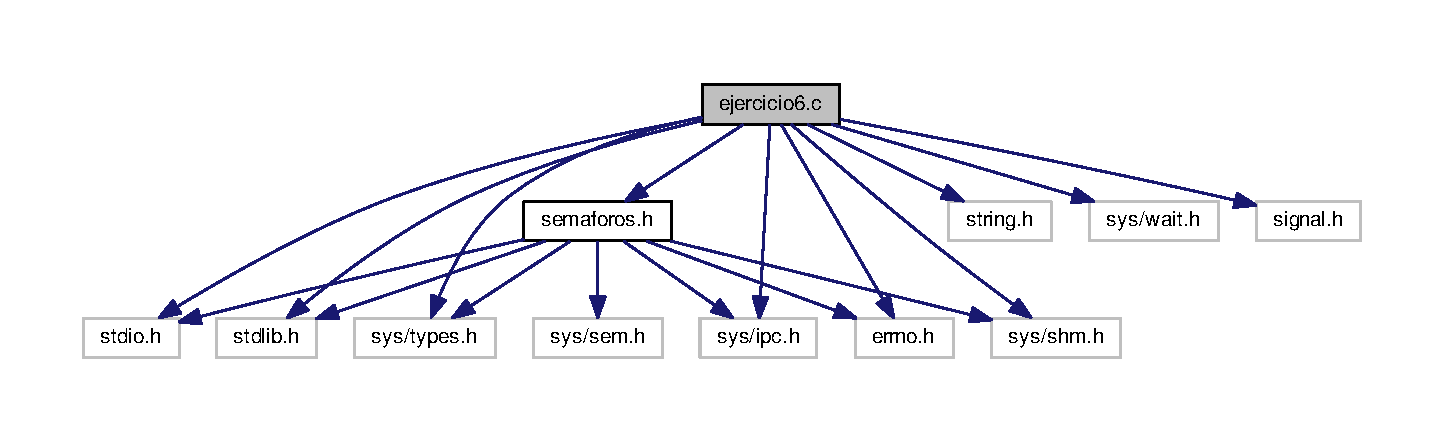
\includegraphics[width=350pt]{ejercicio6_8c__incl}
\end{center}
\end{figure}
\subsection*{Classes}
\begin{DoxyCompactItemize}
\item 
struct \hyperlink{structinfo}{info}
\begin{DoxyCompactList}\small\item\em Variables compartidas. \end{DoxyCompactList}\end{DoxyCompactItemize}
\subsection*{Macros}
\begin{DoxyCompactItemize}
\item 
\#define \hyperlink{ejercicio6_8c_a68c15c5fb7f7c6f707903e6a46ab0557}{F\+I\+L\+E\+K\+E\+Y}~\char`\"{}/bin/cat\char`\"{}
\item 
\#define \hyperlink{ejercicio6_8c_a8ae9d53f33f46cfcfcb9736e6351452a}{K\+E\+Y}~1300
\item 
\#define \hyperlink{ejercicio6_8c_a0240ac851181b84ac374872dc5434ee4}{N}~100
\end{DoxyCompactItemize}
\subsection*{Functions}
\begin{DoxyCompactItemize}
\item 
void \hyperlink{ejercicio6_8c_a52fb52fc24949b9c5e24d67f8249e0bb}{cruzando} (pid\+\_\+t pid, int dir)
\begin{DoxyCompactList}\small\item\em cruzando Imprime por pantalla cuando empieza y termina de usar el recurso \end{DoxyCompactList}\item 
void \hyperlink{ejercicio6_8c_a399eb5cae3f6bbedf44139db5c6c746a}{light\+Switch\+On} (int id\+Mutex, int id\+Recurso, \hyperlink{structinfo}{info} $\ast$buffer, int dir)
\begin{DoxyCompactList}\small\item\em light\+Switch\+On Para pedir el uso del recurso \end{DoxyCompactList}\item 
void \hyperlink{ejercicio6_8c_a69738f15e3376259e4a558cc55e49bd1}{light\+Switch\+Off} (int id\+Mutex, int id\+Recurso, \hyperlink{structinfo}{info} $\ast$buffer, int dir)
\begin{DoxyCompactList}\small\item\em light\+Switch\+Off Indicar que ya has usado el recurso \end{DoxyCompactList}\item 
\hyperlink{ejercicio6_8c_acf22f90c8a4451fe10db34ea170451b5}{coche} (int id\+Mut, int id\+Rec, \hyperlink{structinfo}{info} $\ast$buffer, int dir)
\begin{DoxyCompactList}\small\item\em coche Lo que realiza cada proceso simula que es un coche y quiere cruzar un puente(recurso) \end{DoxyCompactList}\item 
int \hyperlink{ejercicio6_8c_a0ddf1224851353fc92bfbff6f499fa97}{main} (int argc, char $\ast$argv\mbox{[}$\,$\mbox{]})
\begin{DoxyCompactList}\small\item\em Varios procesos compiten por un recurso Se creean 100 procesos, 50 se les asigna una direccion y los otros la otra, y compiten por el uso de un recurso. \end{DoxyCompactList}\end{DoxyCompactItemize}


\subsection{Detailed Description}
El ejercicio 6 de la Practica 3 S\+O\+P\+E\+R. 

\begin{DoxyAuthor}{Author}
Oscar Garcia de Lara Parreño 

Santiago Gomez Aguirre 
\end{DoxyAuthor}
\begin{DoxyVersion}{Version}
1.\+0 
\end{DoxyVersion}
\begin{DoxyDate}{Date}
28-\/03-\/2016 
\end{DoxyDate}


\subsection{Macro Definition Documentation}
\hypertarget{ejercicio6_8c_a68c15c5fb7f7c6f707903e6a46ab0557}{\index{ejercicio6.\+c@{ejercicio6.\+c}!F\+I\+L\+E\+K\+E\+Y@{F\+I\+L\+E\+K\+E\+Y}}
\index{F\+I\+L\+E\+K\+E\+Y@{F\+I\+L\+E\+K\+E\+Y}!ejercicio6.\+c@{ejercicio6.\+c}}
\subsubsection[{F\+I\+L\+E\+K\+E\+Y}]{\setlength{\rightskip}{0pt plus 5cm}\#define F\+I\+L\+E\+K\+E\+Y~\char`\"{}/bin/cat\char`\"{}}}\label{ejercicio6_8c_a68c15c5fb7f7c6f707903e6a46ab0557}
Fichero para sacar la key \hypertarget{ejercicio6_8c_a8ae9d53f33f46cfcfcb9736e6351452a}{\index{ejercicio6.\+c@{ejercicio6.\+c}!K\+E\+Y@{K\+E\+Y}}
\index{K\+E\+Y@{K\+E\+Y}!ejercicio6.\+c@{ejercicio6.\+c}}
\subsubsection[{K\+E\+Y}]{\setlength{\rightskip}{0pt plus 5cm}\#define K\+E\+Y~1300}}\label{ejercicio6_8c_a8ae9d53f33f46cfcfcb9736e6351452a}
Numero para sacar la key \hypertarget{ejercicio6_8c_a0240ac851181b84ac374872dc5434ee4}{\index{ejercicio6.\+c@{ejercicio6.\+c}!N@{N}}
\index{N@{N}!ejercicio6.\+c@{ejercicio6.\+c}}
\subsubsection[{N}]{\setlength{\rightskip}{0pt plus 5cm}\#define N~100}}\label{ejercicio6_8c_a0240ac851181b84ac374872dc5434ee4}
Numero de procesos a crear 

\subsection{Function Documentation}
\hypertarget{ejercicio6_8c_acf22f90c8a4451fe10db34ea170451b5}{\index{ejercicio6.\+c@{ejercicio6.\+c}!coche@{coche}}
\index{coche@{coche}!ejercicio6.\+c@{ejercicio6.\+c}}
\subsubsection[{coche}]{\setlength{\rightskip}{0pt plus 5cm}coche (
\begin{DoxyParamCaption}
\item[{int}]{id\+Mut, }
\item[{int}]{id\+Rec, }
\item[{{\bf info} $\ast$}]{buffer, }
\item[{int}]{dir}
\end{DoxyParamCaption}
)}}\label{ejercicio6_8c_acf22f90c8a4451fe10db34ea170451b5}


coche Lo que realiza cada proceso simula que es un coche y quiere cruzar un puente(recurso) 


\begin{DoxyParams}{Parameters}
{\em id\+Mutex} & id del semaforo mutex \\
\hline
{\em id\+Recurso} & id del semaforo del recurso \\
\hline
{\em $\ast$buffer} & direccion para acceder a las variables compartidas \\
\hline
{\em dir} & dirrecion de donde parte el proceso \\
\hline
\end{DoxyParams}
\hypertarget{ejercicio6_8c_a52fb52fc24949b9c5e24d67f8249e0bb}{\index{ejercicio6.\+c@{ejercicio6.\+c}!cruzando@{cruzando}}
\index{cruzando@{cruzando}!ejercicio6.\+c@{ejercicio6.\+c}}
\subsubsection[{cruzando}]{\setlength{\rightskip}{0pt plus 5cm}void cruzando (
\begin{DoxyParamCaption}
\item[{pid\+\_\+t}]{pid, }
\item[{int}]{dir}
\end{DoxyParamCaption}
)}}\label{ejercicio6_8c_a52fb52fc24949b9c5e24d67f8249e0bb}


cruzando Imprime por pantalla cuando empieza y termina de usar el recurso 


\begin{DoxyParams}{Parameters}
{\em pid} & pid del proceso \\
\hline
{\em dir} & dirrecion de donde parte el proceso \\
\hline
\end{DoxyParams}
\hypertarget{ejercicio6_8c_a69738f15e3376259e4a558cc55e49bd1}{\index{ejercicio6.\+c@{ejercicio6.\+c}!light\+Switch\+Off@{light\+Switch\+Off}}
\index{light\+Switch\+Off@{light\+Switch\+Off}!ejercicio6.\+c@{ejercicio6.\+c}}
\subsubsection[{light\+Switch\+Off}]{\setlength{\rightskip}{0pt plus 5cm}void light\+Switch\+Off (
\begin{DoxyParamCaption}
\item[{int}]{id\+Mutex, }
\item[{int}]{id\+Recurso, }
\item[{{\bf info} $\ast$}]{buffer, }
\item[{int}]{dir}
\end{DoxyParamCaption}
)}}\label{ejercicio6_8c_a69738f15e3376259e4a558cc55e49bd1}


light\+Switch\+Off Indicar que ya has usado el recurso 


\begin{DoxyParams}{Parameters}
{\em id\+Mutex} & id del semaforo mutex \\
\hline
{\em id\+Recurso} & id del semaforo del recurso \\
\hline
{\em $\ast$buffer} & direccion para acceder a las variables compartidas \\
\hline
{\em dir} & dirrecion de donde parte el proceso \\
\hline
\end{DoxyParams}
\hypertarget{ejercicio6_8c_a399eb5cae3f6bbedf44139db5c6c746a}{\index{ejercicio6.\+c@{ejercicio6.\+c}!light\+Switch\+On@{light\+Switch\+On}}
\index{light\+Switch\+On@{light\+Switch\+On}!ejercicio6.\+c@{ejercicio6.\+c}}
\subsubsection[{light\+Switch\+On}]{\setlength{\rightskip}{0pt plus 5cm}void light\+Switch\+On (
\begin{DoxyParamCaption}
\item[{int}]{id\+Mutex, }
\item[{int}]{id\+Recurso, }
\item[{{\bf info} $\ast$}]{buffer, }
\item[{int}]{dir}
\end{DoxyParamCaption}
)}}\label{ejercicio6_8c_a399eb5cae3f6bbedf44139db5c6c746a}


light\+Switch\+On Para pedir el uso del recurso 


\begin{DoxyParams}{Parameters}
{\em id\+Mutex} & id del semaforo mutex \\
\hline
{\em id\+Recurso} & id del semaforo del recurso \\
\hline
{\em $\ast$buffer} & direccion para acceder a las variables compartidas \\
\hline
{\em dir} & dirrecion de donde parte el proceso \\
\hline
\end{DoxyParams}
\hypertarget{ejercicio6_8c_a0ddf1224851353fc92bfbff6f499fa97}{\index{ejercicio6.\+c@{ejercicio6.\+c}!main@{main}}
\index{main@{main}!ejercicio6.\+c@{ejercicio6.\+c}}
\subsubsection[{main}]{\setlength{\rightskip}{0pt plus 5cm}int main (
\begin{DoxyParamCaption}
\item[{int}]{argc, }
\item[{char $\ast$}]{argv\mbox{[}$\,$\mbox{]}}
\end{DoxyParamCaption}
)}}\label{ejercicio6_8c_a0ddf1224851353fc92bfbff6f499fa97}


Varios procesos compiten por un recurso Se creean 100 procesos, 50 se les asigna una direccion y los otros la otra, y compiten por el uso de un recurso. 

\begin{DoxyReturn}{Returns}
E\+X\+I\+T\+\_\+\+F\+A\+I\+L\+U\+R\+E en caso de error, E\+X\+I\+T\+\_\+\+S\+U\+C\+C\+E\+S\+S si funciona 
\end{DoxyReturn}

\hypertarget{semaforos_8h}{\section{semaforos.\+h File Reference}
\label{semaforos_8h}\index{semaforos.\+h@{semaforos.\+h}}
}


\hyperlink{semaforos_8h}{semaforos.\+h}  


{\ttfamily \#include $<$sys/types.\+h$>$}\\*
{\ttfamily \#include $<$sys/ipc.\+h$>$}\\*
{\ttfamily \#include $<$sys/sem.\+h$>$}\\*
{\ttfamily \#include $<$sys/shm.\+h$>$}\\*
{\ttfamily \#include $<$errno.\+h$>$}\\*
{\ttfamily \#include $<$stdio.\+h$>$}\\*
{\ttfamily \#include $<$stdlib.\+h$>$}\\*
{\ttfamily \#include $<$signal.\+h$>$}\\*
{\ttfamily \#include $<$unistd.\+h$>$}\\*
Include dependency graph for semaforos.\+h\+:
\nopagebreak
\begin{figure}[H]
\begin{center}
\leavevmode
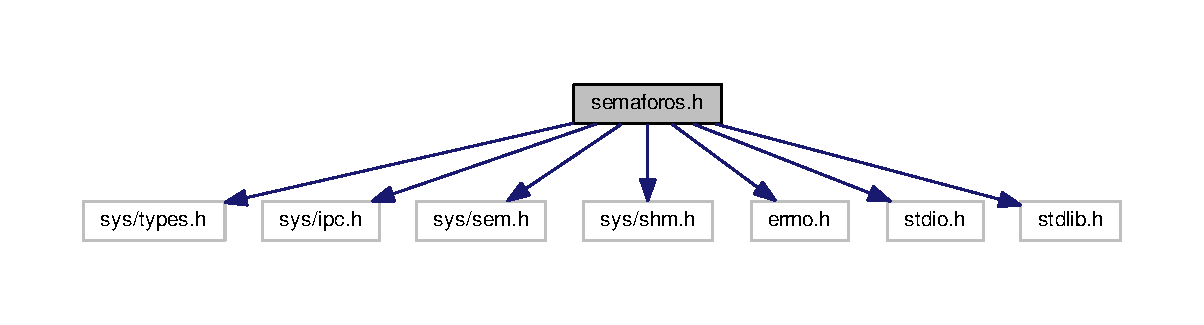
\includegraphics[width=350pt]{semaforos_8h__incl}
\end{center}
\end{figure}
This graph shows which files directly or indirectly include this file\+:
\nopagebreak
\begin{figure}[H]
\begin{center}
\leavevmode
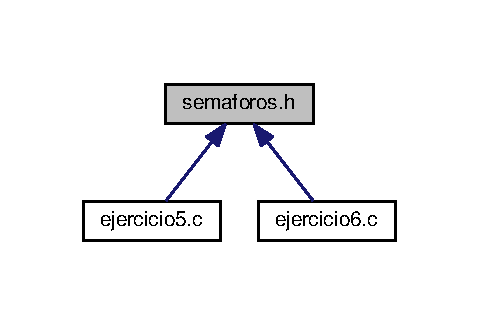
\includegraphics[width=288pt]{semaforos_8h__dep__incl}
\end{center}
\end{figure}
\subsection*{Classes}
\begin{DoxyCompactItemize}
\item 
struct \hyperlink{struct__Mensaje}{\+\_\+\+Mensaje}
\begin{DoxyCompactList}\small\item\em Mensaje. \end{DoxyCompactList}\item 
struct \hyperlink{structAula}{Aula}
\begin{DoxyCompactList}\small\item\em \hyperlink{structAula}{Aula}. \end{DoxyCompactList}\end{DoxyCompactItemize}
\subsection*{Typedefs}
\begin{DoxyCompactItemize}
\item 
typedef struct \hyperlink{struct__Mensaje}{\+\_\+\+Mensaje} \hyperlink{semaforos_8h_a0b62810db7104177e9427c356d59277e}{mensaje}
\begin{DoxyCompactList}\small\item\em Mensaje. \end{DoxyCompactList}\end{DoxyCompactItemize}
\subsection*{Enumerations}
\begin{DoxyCompactItemize}
\item 
\hypertarget{semaforos_8h_a32c27cc471df37f4fc818d65de0a56c4}{enum {\bfseries S\+T\+A\+T\+U\+S} \{ {\bfseries O\+K} =0, 
{\bfseries E\+R\+R\+O\+R} =-\/1
 \}}\label{semaforos_8h_a32c27cc471df37f4fc818d65de0a56c4}

\end{DoxyCompactItemize}
\subsection*{Functions}
\begin{DoxyCompactItemize}
\item 
\hypertarget{semaforos_8h_a4af104b0ed37e6ae0289a1059bc6e990}{int {\bfseries Inicializar\+\_\+\+Semaforo} (int semid, unsigned short $\ast$array)}\label{semaforos_8h_a4af104b0ed37e6ae0289a1059bc6e990}

\item 
\hypertarget{semaforos_8h_a731339337960a681efa435a10f12c312}{int {\bfseries Borrar\+\_\+\+Semaforo} (int semid)}\label{semaforos_8h_a731339337960a681efa435a10f12c312}

\item 
\hypertarget{semaforos_8h_a16b16dd895b5f4cbe48f1ac8977e8b35}{int {\bfseries Crear\+\_\+\+Semaforo} (key\+\_\+t key, int size, int $\ast$semid)}\label{semaforos_8h_a16b16dd895b5f4cbe48f1ac8977e8b35}

\item 
\hypertarget{semaforos_8h_a883244cd3b83c42cda23687da1b63369}{int {\bfseries Down\+\_\+\+Semaforo} (int id, int num\+\_\+sem, int undo)}\label{semaforos_8h_a883244cd3b83c42cda23687da1b63369}

\item 
\hypertarget{semaforos_8h_ab375ebfc38acbdced46e062a689d5fad}{int {\bfseries Down\+Multiple\+\_\+\+Semaforo} (int id, int size, int undo, int $\ast$active)}\label{semaforos_8h_ab375ebfc38acbdced46e062a689d5fad}

\item 
\hypertarget{semaforos_8h_a2d5e735aecee4f493898b3d4ebab1a10}{int {\bfseries Up\+\_\+\+Semaforo} (int id, int num\+\_\+sem, int undo)}\label{semaforos_8h_a2d5e735aecee4f493898b3d4ebab1a10}

\item 
\hypertarget{semaforos_8h_a943759695f018d64a94b8a2c49308092}{int {\bfseries Up\+Multiple\+\_\+\+Semaforo} (int id, int size, int undo, int $\ast$active)}\label{semaforos_8h_a943759695f018d64a94b8a2c49308092}

\end{DoxyCompactItemize}


\subsection{Detailed Description}
\hyperlink{semaforos_8h}{semaforos.\+h} 

\begin{DoxyAuthor}{Author}
Oscar Garcia de Lara Parreño 

Santiago Gomez Aguirre 
\end{DoxyAuthor}
\begin{DoxyVersion}{Version}
1.\+0 
\end{DoxyVersion}
\begin{DoxyDate}{Date}
29-\/03¡4-\/2016 
\end{DoxyDate}


\subsection{Typedef Documentation}
\hypertarget{semaforos_8h_a0b62810db7104177e9427c356d59277e}{\index{semaforos.\+h@{semaforos.\+h}!mensaje@{mensaje}}
\index{mensaje@{mensaje}!semaforos.\+h@{semaforos.\+h}}
\subsubsection[{mensaje}]{\setlength{\rightskip}{0pt plus 5cm}typedef struct {\bf \+\_\+\+Mensaje} {\bf mensaje}}}\label{semaforos_8h_a0b62810db7104177e9427c356d59277e}


Mensaje. 

Esta estructura define un mensaje. 
%--- End generated contents ---

% Index
\newpage
\phantomsection
\addcontentsline{toc}{chapter}{Index}
\printindex

\end{document}
